\chapter{مفاهیم}
\section{اینترنت اشیا}
اینترنت اشیا که از آن به عنوان انقلاب صنعتی جدید یاد می‌شود، به دلیل تغییری که در شیوه زندگی، کار، سرگرمی و مسافرت مردم و ... ایجاد کرده، تعاملات بین دولت‌ها و دنیای پیرامون‌شان را با دنیای مجازی و تكنولوژی نیز دگرگون ساخته است. ورود دستگاه اتومبیل با مجموعه‌ای از نرم‌افزارهای کاربردی جهت ایجاد تعامل بین کاربر، خانه‌ها و ساختمان‌های هوشمند، امكان پخش موسیقی تنها با ادای چند کلمه و هزاران کاربرد دیگر در مدیریت هوشمند شهر، حمل و نقل، کشاورزی، صنایع دفاعی،
صنعت بیمه، صنایع مربوط به نفت، گاز و معدن، مدیریت انرژی، پایش و امنیت اماکن عمومی و
خصوصی، خرده فروشی، بانک‌ها، بهداشت و درمان، هتل‌داری، مهر تاییدی بر اهمیت اینترنت اشیا است.


اینترنت اشیا، برای نخستین بار در سال ۱۹۹۹ توسط کوین اشتون مورد استفاده قرار گرفت و جهانی را توصیف کرد که در آن هر چیزی، از جمله اشیا بی‌جان، برای خود هویت دیجیتال داشته باشند و به کامپیوترها اجازه دهند تا آن ها را سازماندهی و مدیریت کنند \cite{Madakam2015}.


در سال‌های بعد، تعاریف دیگری از اینترنت اشیا توسط افراد و شرکت‌های مختلف ارائه گردید. اینترنت اشیا مفهومی جدید در دنیای فناوری و ارتباطات است که به طور خلاصه می‌توان گفت، اینترنت اشیا فناوری مدرنی است که در آن برای هر موجودی (انسان، حیوان و یا اشیا) قابلیت ارسال داده از طریق شبكه‌های ارتباطی، اعم از اینترنت یا اینترانت، فراهم می‌گردد. در این فناوری، اشیا پیرامون ما قادرند از محیط اطراف خود داده‌های مفیدی را از طریق حسگرهای مختلف جمع‌آوری کرده و آن‌ها را برای پردازش و اتخاذ تصمیمات لازم به یک سیستم مرکزی منتقل کنند. در واقع ایده کلی فناوری اینترنت اشیا دریافت، ذخیره‌سازی و ارسال اطلاعات از محیط به منظور تحلیل آن‌ها و در نهایت ارائه خدمات بهتر و هوشمندتر به کاربر نهایی است. به عبارتی اینترنت اشیا را می‌توان به عنوان تكامل بعدی اینترنت دانست که جهش بزرگی در توانایی جمع‌آوری، تحلیل و توزیع داده دارد.


اینترنت اشیا یک شبكه داخلی متشکل از دستگاه‌های فیزیکی، وسایل نقلیه، ساختمان‌ها، سایر موارد الكترونیكی، نرم‌افزارها، حسگرها، محرك‌ها و یک اتصال به شبكه که اشیا را به جمع‌آوری و تبادل
داده‌ها قادر می‌سازد، می‌باشد. در سال ۲۰۱۳ میلادی استانداردهای جهانی، برای اینترنت اشیا تعریف "زیرساخت‌های جامعه اطلاعاتی" را مطرح کردند. اینترنت اشیا امكان حس و کنترل شدن اشیا از راه دور را با استفاده از زیرساخت شبكه فراهم می‌سازد، فرصت ادغام مستقیم دنیای فیزیكی با سیستم‌های کامپیوتری را بالا می‌برد و در نتیجه بهبود بهره‌وری، دقت و سود اقتصادی را علاوه بر کاهش دخالت انسان به همراه دارد.
\subsection{سیر تکامل}
تغییراتی که در تعامل و ارتباطات بین موجودیت‌های (اشیای) موجود در جهان، در طول زمان (قبل از ظهور اینترنت، بعد از ظهور آن تا مطرح شدن ایده اینترنت اشیا) بوجود آمده، در شكل ۲-۱ به
تصویر کشیده شده است:
\begin{figure}[!h]
	\centerline{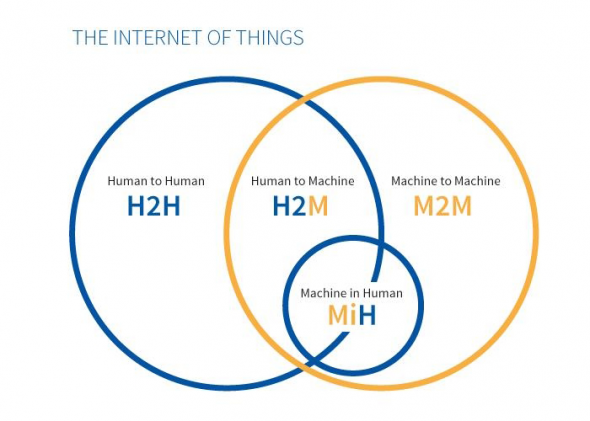
\includegraphics[width=.7\textwidth]{iot-m2m}}
	\caption{سیر تکامل ارتباطات موجودیت‌های جهان \cite{connection}}
\end{figure}

تكامل در ارتباطات شامل مراحل زیر است:
\begin{enumerate}
	\item
	 قبل از اینترنت: ارتباط انسان با انسان
	\item
	اینترنت محتوا: وب نسل ۱ بر روی بستر شبکه‌های \lr{IP}
	\item 
	اینترنت سرویس: وب نسل ۲ و امکان تولید محتوا توسط کاربران
	\item 
	اینترنت افراد: شبکه‌ها و رسانه‌های اجتماعی
	\item
	اینترنت اشیا: اتصالات ماشین به ماشین
\end{enumerate}


ارتباطات ماشین به ماشین \RTLfootnote{\lr{M2M}} اصطلاحی است که برای توصیف هر فناوری که دستگاه‌های شبكه را قادر به تبادل اطلاعات و انجام برخی عملیات بدون دخالت انسان می‌کند، به کار گرفته می‌شود. در واقع به عنوان بخشی از اینترنت اشیا در نظر گرفته می‌شود. پیش‌بینی‌ها نشان می‌دهد که تعداد اتصالات اینترنت اشیا در سال‌های آینده رشد قابل توجهی خواهد داشت.


مفاهیم مرتبط به اینترنت اشیا سال‌ها قبل توسط مارك ویسر در شرکت زیراکس مطرح شده بود و
در قالب حوزه پردازش فراگیر در حال رشد بود. هدف حوزه پردازش فراگیر شكل‌گیری جهانی است که در آن اشیا اطراف ما (که به طور روزمره با آن‌ها سر و کار داریم) دارای قدرت پردازش بوده و به
صورت بی‌سیم یا کابلی با شبكه جهانی در ارتباط باشند. دورنمای دیدگاه اولیه مارك ویسر دستیابی به سیستم‌های شبكه‌ای در حوزه فناوری اطلاعات و ارتباطات است که نهفته در محیط پیرامون، پنهان از دید کاربر و خودکار هستند. چنین سیستم‌هایی کاربر و فعالیت‌هایش را دنبال کرده و به نیازمندی‌های آن پاسخ می‌دهد. لذا به عبارتی کاربر را قادر می‌سازد با محیط فیزیكی اطرافش سازگار شود و سرویس هوشمندتری را دریافت کند.

\subsection{اکوسیستم}
با توجه به تعاملی که اینترنت اشیا بین عناصر و اشیا متنوع ایجاد کرده و با درنظر گرفتن این موضوع که فناوری‌های اینترنت اشیا مختص یک صنعت و یا زنجیره تامین خاصی نیستند، این مسئله باعث ایجاد روابط پیچیده‌ای می‌شود که شامل تعداد زیادی از بازیگران خواهد بود. در این صورت بایستی با استفاده از مفهوم اکوسیستم، به این شرایط پیچیده سامان بخشید.


هدف اینترنت اشیا قابلیت‌ بخشی به اشیا برای ارتباط با هم در همه جا، هر زمان و با هر وسیله، راه و شبكه‌ ارتباطی است. با این وجود اینترنت اشیا، تعامل چند دنیا است که دارای اجزای مختلفی است که خود حاصل تعامل سه دنیا است و گاها از این سه دنیا تحت عنوان اجزای اینترنت اشیا نیز یاد می‌شود که عبارتند از:
\begin{enumerate}
	\item دنیای دیجیتال
	\item دنیای سایبری
	\item دنیای فیزیکی واقعی
\end{enumerate}
\subsection{معماری فنی اینترنت اشیا}
اینترنت اشیا، ارتباطات ماشین به ماشین، وب فیزیكی و فناوری‌های متعدد دیگری که با توسعه شبكه‌های ارتباطی و تكنولوژی‌های تجمیع و تحلیل داده‌ها در سال‌های اخیر به آن‌ها پرداخته می‌شود، عملا یک هدف ثابت را دنبال می‌کنند. این هدف بكارگیری هوشمند داده‌های تولیدی از ابزارهای متصل به شبكه و سابقه قبلی اتصال آنها با هدف ارائه سرویس بهتر به مشتریان انتهایی است.\\
 معماری اصلی این سرویس‌ها را می‌توان به بخش‌های زیر تقسیم‌بندی کرد:
\begin{itemize}
	\item سخت‌افزار (شامل حسگرها، عملگرها و دروازه‌های اتصال به شبکه)
	\item شبکه مخابراتی ارتباطی (شامل شبکه انتقال مبتنی بر دسترسی)
	\item بستر ابری و مدیریت سرویس (مرکز داده، پلتفرم تحلیل کلان داده و میان‌افزار ارائه سرویس)
	\item برنامه‌های کاربردی (شامل توسعه‌دهندگان سرویس و سرویس گیرندگان)
\end{itemize}
این معماری چند لایه‌ای در شكل زیر نشان داده شده است:\\
\begin{figure}[!h]
	\centerline{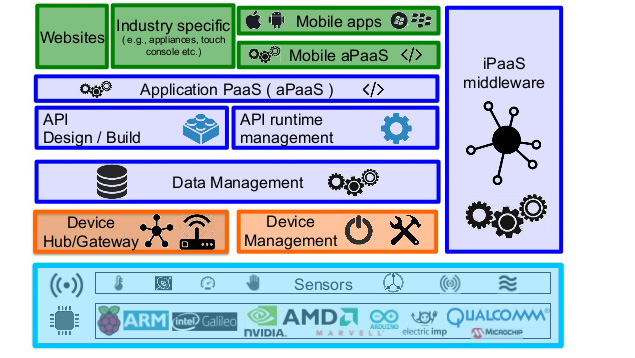
\includegraphics[width=.8\textwidth]{iot-arc}}
	\caption{معماری اینترنت اشیا \cite{iot-arc}}
\end{figure}

\subsection{کاربردها}
سرویس‌ها و کاربردهای اینترنت اشیا در حوزه‌های متنوعی مطرح هستند، که از آن جمله می‌توان به این موارد اشاره کرد: ساختمان، انرژی، خانه و مشتری، سلامت، صنعت حمل و نقل، امنیت عمومی، شبكه و فناوری اطلاعات. میزان محبوبیت کاربردهای این حوزه متفاوت است. محبوب‌ترین کاربردها به ترتیب عبارتند از: ابزارهای پوششی، شهر هوشمند، خانه هوشمند، اینترنت صنعتی، توزیع هوشمند برق، سلامت، کشاورزی و دامپروری، زنجیره تامین
\section{سیستم ردیابی}
همانطور که گفتیم اینترنت اشیا چهارچوبی است که در آن هر شی دارای قابلیت اتصال به اینترنت است.
	این اتصال به اینترنت دستگاه‌های محاسباتی تعبیه شده در هر شی، آن را قادر به ارسال و دریافت اطلاعات می‌کند. اینترنت اشیا به طور گسترده به گسترش ارتباط شبکه‌ای و قابلیت محاسبه اشیا، دستگاه‌ها، حسگرها و هر چیزی که به طور عادی کامپیوتر حساب نمی‌شود، اشاره دارد. کوین اشتون، پدر اینترنت اشیا، اشاره می‌کند که "اطلاعات و داده‌ها راه عالی برای کاهش هدرروی و افزایش بهره‌وری می‌باشد و این دقیقا آن چیزی است که اینترنت اشیا فراهم می‌کند." این اشیا هوشمند دارای حداقل نیاز انسان برای تولید، مبادله و محاسبه داده می‌باشند. زمینه‌های کاربرد تکنولوژی اینترنت اشیا روز به روز در حال افزایش است. یکی از کاربردهای اینترنت اشیا در ردیابی وسایل نقلیه است \cite{Mangla2017, Mukhtar2015}.
	
انتظار می‌رود تعداد کل وسایل نقلیه روز به روز افزایش یابد با توجه به اینکه مالکیت آن‌ها برای افراد با توحه به اقتصاد رو به رشد کشورهایی مثل چین و هند، مقرون به صرفه می‌باشد. اما با این وجود کمبود سیستم ردیابی هم‌چنان حس می‌شود. چنین سیستمی در زمینه‌های مختلفی از چمله امنیت خودرو شخصی، وسایل نقلیه عمومی، مدیریت ناوگان و ... کاربرد دارد \cite{Pham2013}. امروزه سیستم‌های ردیابی مختلفی در بازار وجود دارد اما آن‌ها دارای کاربرد مشخص، ناحیه کاری مشخص و عمدتا هم بسیار هزینه‌بر می‌باشند \cite{YoujingCui2003}. بنابراین سیستم ردیابی طراحی شده برای امنیت خودرو برای مدیریت ناوگان مناسب نمی‌باشد \cite{Song2008}. پس باید سیستمی را پیاده‌سازی کنیم که به راحتی برای کاربردهای مختلف قابل استفاده و مقرون به صرفه باشد.


همانطور که اشاره کردیم سیستم ردیابی راه‌حلی برای مدیریت ناوگان و امنیت اشیا متحرک از جمله افراد، وسایل نقلیه و ... می‌باشد. این تکنولوژی برای مشخص کردن مکان شی متحرک در هر زمان از متدهای مختلفی مثل سیستم موقعیت‌یاب جهانی \RTLfootnote{\lr{GPS}} که به ماهواره‌های اطراف پایگاه زمین متصل می‌باشد، استفاده می‌کند. سیستم‌های ردیابی مدرن از تکنولوژی جی پی اس برای مانیتور و موقعیت‌یابی وسایل نقلیه در هر کجای زمین استفاده می‌کنند. این سیستم ردیابی در داخل خودرو یا هر شی متحرکی که می‌خواهیم آن را ردیابی کنیم، قرار می‌گیرد و امکان موقعیت‌یابی در هر لحظه را فراهم می‌آورد  و اطلاعات لازم برای ردیابی را در اختیار افراد می‌گذارد. این سیستم یک دستگاه ضروری برای ردیابی اشیا متحرک مخصوصا وسایل نقلیه است که صاحبان آن‌ها بتوانند هر زمان وسیله نقلیه خود را ردیابی کنند. هم‌چنین از این سیستم می‌توان برای ردیابی و پیدا کردن وسایل دزدیده شده استفاده نمود. داده جمع‌آوری شده از طریق این سیستم را می‌توان بر روی نقشه الکترونیکی از طریق اینترنت یا نرم‌افزارهای کاربردی مشاهده نمود.


سیستم ردیابی متشکل از اجزای سخت‌ افزاری و نرم ‌افزاری است که با کمک آن‌ها می‌توان شی مورد نظر را ردیابی کرد. این سیستم از سه بخش اصلی تشکیل شده است: شی متحرک، بخش سخت‌افزاری و بخش نرم‌افزاری.
بخش سخت‌افزاری متشکل از برد آردوینو، آنتن جی پی اس و جی اس ام متصل به ماژول سیم ۸۰۸ \RTLfootnote{\lr{SIM808}} در داخل شی که قراره ردیابی شود، قرار می‌گیرد. این بخش سیگنال حاوی مختصات مکانی و زمانی است را به کمک آنتن جی پی اس از ماهواره دریافت می‌کند. مودم جی اس ام این اطلاعات را به سرور می‌فرستد که پس از دریافت و تحلیل بر روی نقشه می‌توان مسیر حرکت را مشاهده نمود.


 یکی از نگرانی‌های اصلی صاحبان وسیله نقلیه، امنیت آن‌ها می‌باشد. از این رو همواره به دنیال سیستم امنیتی جدید و کارآمد هستند. با پیشرفت تکنولوژی امروزه قادر خواهیم بود در هر زمان وسیله نقلیه را ردیابی و موقعیت آن را در هر لحظه مشاهده کنیم. سیستم ردیابی با استفاده از ردیابی  کردن فعالیت‌های وسیله نقلیه در بازه‌های زمانی مشخص کمک بسزایی در تامین امنیت آن‌ها کرده است. این سیستم از جی پی اس برای پیدا کردن اطلاعات مربوط به مکان هر شی استفاده می‌کند و سپس  این اطلاعات برای نمایش مسیر حرکت به سرور فرستاده می‌شوند.
 
 
 بخش سخت‌افزاری سیستم ردیابی در داخل وسیله نقلیه به نحوی قرار می‌گیرد که از بیرون آن قابل مشاهده نباشد. درواقع به عنوان یه بخش پنهان شده عمل می‌کند که به طور مداوم مختصات مکانی شی را به سرور می‌فرستد.
 در سمت سرور برنامه کاربردی تحت وب توسعه داده می‌شود که این امکان را فراهم می‌کند  مسیر حرکت شی را بر روی نقشه مشاهده کرد.
 
 سیستم ردیابی بزرگترین پیشرفت تکنولوژی در زمینه تامین امنیت می‌باشد. این سیستم صاحبان وسال نقلیه را قادر می‌سازد بتوانند از راه دور در هر زمانی وسیله نقلیه خویش را ردیابی کنند.
 
 
 سیستم ردیابی هم‌چنین به عنوان دستگاه پیشگیری از سرقت و بازیابی وسیله نقلیه در میان مردم مشهور شده است. وقتی وسیله نقلیه دزدیده می‌شود، اطلاعات ارسال شده توسط سیستم ردیابی را می‌توان در اختیار پلیس گذاشت تا آن‌ها به راحتی با دنیال کردن سیگنال‌های دریافتی موقعیت علی وسیله نقلیه موردنظر را پیدا کنند.
 
 
 سیستم ردیابی زمانی که به عنوان یک سیستم امنیتی مورد استفاده قرار می‌گیرد، می‌تواند حایگرین مناسبی برای سیستم‌های هسشدار دهنده سنتی خودروها باشد. برخی از سیستم‌های ردیابی قادر هستند از راه دور وسیله نقلیه را کنترل کنند که این کنترل شامل قفل کردن در خودرو و خاموش کردن موتور آن در موارد اضطراری می‌باشد. با توجه به پیشرفت روزافزون تکنولوژی، سیستم ردیابی قادر هستند که حرکت غیر عادی وسیله نقلیه را تشخیص داده و به صاحب آن هشدار دهند.
 
  
  سیستم ردیابی در داخل شی که قرار است آن را ردیابی کنیم، قرار می‌گیرد. این شی از طزیق یک تلفن همراه که به کاربر امکان ارتباط از راه دور با سیستم تعبیه شده را فراهم می‌کند. سیستم ردیابی از یک سیم‌کارت برای ارسال و دربافت پیام کوتاه استفاده می‌کند. کاربر می‌تواند با استفاده از تلفن همراه خویش یک پیام کوتاه به سیم‌کارت تعبیه شده در سیستم ردیابی بفرستد و از طریق بتواند وسیله نقلیه خود را ردیابی کند.
به طور کلی عملکرد سیستم ردیابی را میتوان دو بخش کرد:
  \begin{enumerate}
  	\item ردیابی وسیله نقلیه
	\item تامین امنیت وسیله نقلیه
  \end{enumerate}
این سیستم از یک آنتن جی اس ام تشکیل شده است که ردیابی واقعی شی را ممکن می‌سازد. مودم جی اس ام که مستقیما به میکروکنترلر متصل است امکان ارسال و دریافت پیام کوتاه و فرستادن داده به سرور را فراهم می‌کند. این مودم اطلاعات را دریافت می‌کند و آن را به تلفن همراه کاربر که با آن تقاضا دریافت موقعیت مکانی را کرده بود، می‌فرستد. این اطلاعات شامل طول جغرافیایی \RTLfootnote{\lr{Longitude}}، عرض جغرافیایی \RTLfootnote{\lr{Latitude}} به همراه یک لینک می‌باشد که با کلیک کردن بر روی آن می‌توان موقعیت شی را بر روی نقشه مشاهده کرد.
\\
\\
\\
\section{تکنولوژی جی پی اس}
سیستم موقعیت‌‌یاب جهانی توسط دولت و ارتش ایالت متحده آمریکا طراحی شد که از آن برای اهداف نظارتی استفاده می‌کردند. \lr{GPS} توسط وزارت دفاع ایالات متحده آمریکا و دکتر ایوان \RTLfootnote{Dr. Ivan} به عنوان سیستم ناوبری ماهواره‌‌ای اختراع شد.


سیستم موقعیت‌یاب جهانی منظومه‌ای متشکل از ۲۴ ماهواره است که زمین را دور می‌زند و در هر مدار ۴ ماهواره قرار دارد. راکت‌های کوچکی نیز ماهواره‌ها را در مسیر صحیح نگاه می‌دارد. به این ماهواره‌ها نوستار نسز گفته می‌شود.
شناسایی موقعیت جغرافیایی بین ۱۰ تا ۱۰۰ متر را مکان‌پذیر می‌سازد. این ماهواره‌ها از محاسبات ریاضی ساده‌ای برای پخش اطلاعات استفاده می‌کنند که به عنوان طول و عرض و ارتفاع جغرافیایی، توسط گیرنده‌های زمین ترجمه شده‌اند.


سیستم جی‌پی‌اس بدون وابستگی به گیرنده‌های تلفن یا اینترنت عمل می‌کند، اگر چه با این فناوری‌ها می‌توان اطلاعات دریافتی از این سیستم موقعیت‌یابی را مناسب تر و کاربردی تر کرد. سیستم جی‌پی‌اس می‌تواند توانایی‌های حیاتی در زمینه موقعیت‌یابی برای کاربران نظامی، مدنی یا کاربران عادی در سراسر جهان فراهم کند. 


پروژه جی‌پی‌اس در سال ۱۹۷۳ و توسط ایالات متحده، برای غلبه بر محدودیت‌های سیستم‌های موقعیت‌یابی پیشین شروع شد. وزارت دفاع آمریکا سیستمی را توسعه داد که به شکل پیش‌فرض ۲۴ ماهواره را به کار می‌برد. طراحی و توسعه و پشتیبانی این سیستم بر عهده وزارت دفاع ایالات متحده است.


جی‌پی‌اس در تمام شرایط به‌صورت ۲۴ ساعت در شبانه‌روز و در تمام دنیا قابل استفاده‌ است و هیچ‌گونه بهایی بابت این خدمات اخذ نمی‌شود. ماهواره‌های جی‌پی‌اس، هر روز دو بار در یک مدار دقیق دور زمین می‌گردند و سیگنال‌های حاوی اطلاعات را به زمین می‌فرستند.


سیستم‌های مشابهی نیز وجود دارند که در حال استفاده یا طراحی هستند. سیستم روسی گلوناس مهم‌ترین آن‌ها است که تقریباً هم‌زمان با جی‌پی‌اس تکامل یافته اما از سال ۲۰۰۸ به بهره‌برداری کامل رسیده‌ است. اتحادیه اروپا، هند و چین نیز هر یک سیستم‌های مشابهی را در دست توسعه دارند.

\subsection{تاریخچه}
از اوایل دهه ۶۰ میلادی، نیروی هوایی و نیروی دریایی آمریکا همواره در حال مطالعه یا اقدام جهت دستیابی به یک سیستم ناوبری ماهواره‌ای بوده‌اند. نیروی دریایی دو طرح عمده \lr{Transit} و \lr{Timation} را در دست اقدام داشته‌است. \lr{Transit} توسط آزمایشگاه‌های فیزیک کاربردی جان هاپکینز طراحی و در سال ۱۹۶۴ به حالت عملیاتی درآمد. این سیستم اکنون اطلاعات ناوبری سطح را به‌ صورت دو بعدی (طول و عرض جغرافیایی) و بر مبنای اصول شیفت داپلر برای کاربران دریانوردی فراهم می‌آورد. سیستم \lr{Timation}  طرحی تحقیقاتی با فناوری پیشرفته از آزمایشگاه تحقیقات نیروی دریایی آمریکا بود که یک سیستم ناوبری دو بعدی (طول و عرض جغرافیایی) را بر مبنای زمان‌سنجی دقیق ارائه می‌کرد. در همین دوره زمانی، نیروی هوایی نیز تحقیقات پژوهشی را برای ارائه یک سیستم ناوبری سه بعدی (طول و عرض جغرافیایی و ارتفاع) انجام می‌داد. این سیستم بر مبنای فاصله‌یابی ماهواره ای به کمک «دنباله‌های دیجیتال قابل تکرار» و «نویز شبه تصادفی» پایه‌ریزی شده بود

اولین ماهواره جی‌پی‌اس در سال ۱۹۷۸ با موفقیت به فضا پرتاب شد. هدف اصلی و اولیه از طراحی جی‌پی‌اس، اهداف نظامی بوده اما از سال ۱۹۸۰ به بعد برای استفاده‌های غیرنظامی نیز در دسترس قرار گرفت. این سیستم در سال ۱۹۹۵ و با تکمیل تعداد ماهواره‌ها به توان پیش‌بینی شده نهایی خود دست یافت. افتخار اختراع این سیستم به راجر ال استون، ایوان ای گتینگ و برادفورد پارکینسون از آزمایشگاه فیزیک پیشرفته ایالات متحده تعلق دارد.


پیشرفتهای تکنولوژیکی و نیازهای جدید باعث تمایل زیادی برای ارتقا و مدرنیزه کردن سیستم موجود و توسعه نسل جدید ماهواره‌ها با عنوان جی‌پی‌اس بلوک ۳ آ و نسل جدید سیستم‌های کنترل عملیاتی شده‌اند. این تغییرات از سال ۱۹۹۸ با دستور کاخ سفید شروع شدند و در سال ۲۰۰۰ با تصویب کنگره آمریکا شروع به عملیاتی شدن کردند و در نهایت به جی‌پی‌اس نسل سوم خواهند انجامید.
\subsection{ساختار جی‌پی‌اس}
جی‌پی‌اس فعلی از سه بخش اساسی تشکیل شده‌است. این سه بخش اصلی عبارتند از: بخش فضایی، بخش کنترل و بخش کاربر. قسمت‌های کنترل و فضایی توسط نیروی هوایی ایالات متحده آمریکا پایه‌گذاری شده و توسعه یافته‌اند و اکنون نیز به کار خود ادامه می‌دهند. امواج منتشر شده از فضا توسط ماهواره‌های جی‌پی‌اس، توسط گیرنده‌های جی‌پی‌اس دریافت می‌شوند؛ این گیرنده‌ها به وفور در اختیار انواع کاربران قرار دارند و برای محاسبه کردن موقعیت سه بعدی (طول و عرض جغرافیایی و ارتفاع) محل مورد نظر و زمان به کار می‌روند.
\begin{itemize}
	\item
	بخش فضایی: از ۲۴ تا ۳۲ ماهواره تشکیل شده‌ است که در مدار میانی زمین قرار گرفته‌اند و همچنین شامل تأسیساتی هم می‌شود که برای آماده‌سازی و پرتاب آن‌ها به کار می‌روند.
	\item 
	
	بخش کنترل: از یک ایستگاه اصلی کنترل زمینی، یک ایستگاه اصلی کنترل زمینی دیگر به عنوان پشتیبان، یک میزبان آنتن‌های اختصاصی و اشتراکی برای سیستم و ایستگاه‌های پایش تشکیل شده‌است.
	
	\item  
	بخش کاربری: از صدها هزار کاربر نظامی آمریکایی و متحدان آن که از جی‌پی‌اس کدگذاری شده برای تعیین موقعیت دقیق استفاده می‌کنند و صدها میلیون کاربر مدنی، عمومی یا علمی تشکیل شده‌است که از امکانات موقعیت‌یابی استاندارد استفاده می‌کنند.
\end{itemize}
\subsection{بخش فضایی}
بخش فضایی از ماهواره‌های مستقر در مدار زمین تشکیل شده ‌است که به اختصار ماشین‌های فضایی نیز نامیده می‌شوند. در طراحی اولیه جی‌پی‌اس بیست وچهار ماشین فضایی مورد نیاز بود که در هشت  مدار دایره‌ای و در هر مدار حداکثر سه ماهواره قرار می‌گرفتند. بعدها این طرح تبدیل به شش مدار شد و در هر مدار حداکثر چهار ماشین فضایی در نظر گرفته شد.


نقشه شش مداری حداکثر ۵۵ درجه انحراف مداری دارد که هر مدار ۶۰ درجه فاصله از گره نزولی دارد. زمان مداری نصف یک روز نجومی است؛ معنی آن این است که روزانه حدود ۱۱ ساعت و ۵۸ دقیقه طول می‌کشد تا ماهواره از روی مکان قبلی یا تقریباً نزدیک آن عبور کند.


مدارها به شکلی تنظیم شده‌اند که در تمام ساعات شبانه روز و تقریباً از تمام نقاط سطح زمین، حداقل ۶ ماهواره در خط دید باشند. برای تحقق این موضوع فاصله یکسانی برای ماهواره‌های موجود در مدار مشترک در نظر گرفته نشده‌ است. اگر ساده‌تر در نظر بگیریم فاصله زاویه‌ای بین بین ماهواره‌ها به این شکل است: ۳۰،  ۱۰۵،  ۱۲۰،  ۱۰۵ درجه که در مجموع ۳۶۰ درجه می‌شود.


ارتفاع مداری حداکثر حدود ۲۰۲۰۰ کیلومتر است، یعنی شعاع مداری حداکثر ۲۶۶۰۰ کیلومتر است. هر ماشین فضایی، در هر روز نجومی دو بار و همان مسیر قبلی را نسبت به زمین می‌پیماید. این مسئله مخصوصا هنگام ارتقا و تکمیل سیستم خیلی کمک‌ کننده بود چرا که حتی فقط با ۴ ماهواره و جاگیری صحیح، هر چهار ماهواره در طی چند ساعت، از یک نقطه خاص قابل رویت بودند. برای عملیات‌های نظامی، تکرار گذرهای زمینی از یک منطقه می‌تواند منجر به اطمینان از پوشش خوب منطقه نبرد باشد.


در فوریه ۲۰۱۶، ۳۲ ماهواره در سیستم جی‌پی‌اس حضور داشتند که ۳۱ عدد از آن‌ها فعال بودند. ماهواره‌های اضافی دقت محاسبات گیرنده‌های جی‌پی‌اس برای اندازه‌گیری‌های دقیق را افزایش می‌دهند. با افزایش تعداد ماهواره‌ها چینش آن‌ها در مدارها به شکل ناهمسانی تغییر کرد. مزیت این شکل از چینش نسبت به فرم استاندارد این است که در صورت از دست رفتن یکی از ماشینها فضایی (عدم کارکرد صحیح)، در دسترس بودن سیستم کاهش نمی‌یابد و هنوز مورد اعتماد باقی می‌ماند. با وضعیت فعلی از هر نقطه زمین و در هر زمانی در حدود ۹ ماهواره به شکل هم‌زمان در خط دید قرار دارند. این امر باعث افزایش قابل توجه اعتماد به دقت، نسبت به حضور حداقل ۴ ماهواره، برای تعیین مکان می‌شود.
\subsection{کنترل زمینی}
بخش کنترل این بخش شامل ایستگاه‌های کنترل زمینی است که دارای مختصات معلوم هستند و موقعیت آن‌ها از طریق روش‌های کلاسیک تعیین موقعیت نظیر روش تعیین فواصل بلند توسط کوازارها و روش فاصله سنجی ماهواره‌ای با امواج لیزر بدست آمده ‌است. این ایستگاه‌ها وظیفه تعقیب چندجمله‌ایِ ریاضی به طریق کمترین مربعات، پارامترهای مداری و موقعیت ماهواره‌ها را نسبت به یک سیستم مختصات ژئودتیک ژئوسنتریک (مبدأ سیستم مختصات تقریباً در مرکز زمین قرار دارد) محاسبه می‌نماید.
\\
تعداد این ایستگاه‌های زمینی ۵ عدد است که ایستگاه اصلی با نام کلرادو اسپرینگ در آمریکا قرار دارد و ۴ ایستگاه فرعی دیگر در نقاط دیگر کره زمین مستقر هستند. آخرین بخش از سیستم جی‌پی‌اس، قسمتِ کاربران سیستم است که خود شامل دو بخش است:
\begin{enumerate}
	\item آنتن دریافت ‌کننده اطلاعات ارسالی از ماهواره‌ها
	\item گیرنده (پردازش‌کننده اطلاعات دریافتی و تعیین‌کننده موقعیت محل آنتن)
\end{enumerate}
نرم‌افزار و ریزپردازنده داخل گیرنده فاصله بین آنتن زمینی تا ماهواره‌های مرتبط با گیرنده را تعیین می‌کند سپس با استفاده از حداقل ۴ ماهواره موقعیت طول، عرض و ارتفاع محل استقرار آنتن یا همان گیرنده تعیین می‌شود.
نکته مهمی که می‌بایست مورد توجه قرار گیرد این است که ارتفاعی که جی‌پی‌اس به ما می‌دهد با ارتفاع موجود در نقشه‌ها و اطلس‌ها فرق می‌کند. ارتفاع جی‌پی‌اس نسبت به سطح مبنایی به نام بیضوی است در حالی که ارتفاع موجود در نقشه‌ها ارتفاع اورتومتریک است که از سطح دریاهای آزاد محاسبه می‌گردد. مقدار این اختلاف در بیش‌ترین حالت در حدود ۱۰۰ متر است.
\subsection{دقت اندازه‌گیری}
دستگاه‌های جی‌پی‌اس انواع گوناگونی دارند و در وسایل مختلفی استفاده می‌شوند؛ ولی یکی از جاهایی که بیشتر در آن استفاده می‌شود گوشی‌های موبایل است که دقت آن در شرایط مختلف متفاوت است. به عنوان مثال:
\begin{itemize}
	\item فضای باز: ۳ تا ۷ متر
	\item داخل ماشین: ۵ تا ۱۰ متر
	\item داخل خانه دو طبقه: ۲۰ تا ۵۰ متر
	\item داخل آپارتمان: ۵۰۰ تا ۱۰۰۰ متر و در شرایطی قطع
	\item در جنگل: ۱۰۰ تا ۲۰۰ متر
	\item داخل هواپیما: ۵۰ متر
	\item داخل تونل: قطع کامل
	\item بر پشت‌بام آپارتمان: ۲ تا ۴ متر
	\item زیر پل‌ها: قطع کامل
\end{itemize}
\subsection{کاربردها}
اساس کار دستگاه موقعیت‌یاب تعیین موقعیت است و این کار با دریافت امواج ماهواره‌های موقعیت‌یاب که در مدارهایی به دور کره زمین در چرخش هستند، انجام می‌شود. برای تعیین موقعیت، گیرنده موقعیت‌یاب زمان‌های دریافت شده را با زمان خود مقایسه می‌کند. تفاوت این دو مشخص‌کننده فاصله گیرنده موقعیت‌یاب از ماهواره مزبور می‌باشد. این عملی است که دقیقا یک گیرنده موقعیت‌یاب انجام می‌دهد. با استفاده از حداقل سه ماهواره یا بیشتر، موقعیت‌یاب می‌تواند طول و عرض جغرافیایی مکان خود را تعیین نماید. (که آن را تعیین دو بعدی می‌نامند) و با تبادل با چهار (و یا بیشتر) ماهواره یک موقعیت‌یاب می‌تواند موقعیت سه بعدی مکان خود را تعیین نماید که شامل طول و عرض جغرافیایی و ارتفاع می‌باشد. با انجام پشت سر هم این محاسبات، موقعیت‌یاب می‌تواند سرعت و جهت حرکت خود را نیز به دقت مشخص نماید امروزه در بعضی مکان‌های ایران قادر به دریافت اطلاعات تا ۱۰ ماهواره می‌باشیم و حداقل به ۴ تا ۵ ماهواره در هر زمان از شبانه روز و در هر مکان دسترسی داریم. هر قدر تعداد ماهواره‌های قابل مشاهده بیشتر شود معادلات اساسی تعیین موقعیت بیشتر خواهند شد و بنابراین زمان لازم برای تعیین موقعیت یک نقطه کاهش یافته و دقت تعیین موقعیت نیز افزایش خواهد یافت. نکته مهمی که می‌بایست مورد توجه قرار گیرد این است که ارتفاعی که موقعیت‌یاب به ما می‌دهد با ارتفاع موجود در نقشه‌ها و اطلس‌ها فرق می‌کند. ارتفاع موقعیت‌یاب ارتفاع ژئودتیک است که نسبت به سطح مبنایی به نام بیضوی مقایسه اندازه‌گیری می‌شود، در حالی که ارتفاع موجود در نقشه‌ها ارتفاع اورتومتریک یا ارتفاع از سطح ژئوئید می‌باشد که از سطح دریاهای آزاد محاسبه می‌گردد. مقدار اختلاف این دو مقیاس در بیشترین حالت حدود ۱۰۰ متر است. موقعیت‌یاب اطلاعات موقعیتی را توسط اعداد و در یک سیستم مختصاتی بیان می‌کند. 
\\
دستگاه جی‌پی‌اس یک رایانه کوچک است که جهت انجام امور خاصی برنامه‌ریزی شده ‌است؛ بنابراین این رایانه با داشتن مختصات شما می‌تواند کارهای دیگری هم انجام بدهد. مثلا می‌تواند زمان طلوع و غروب خورشید را در موقعیت شما بگوید. همچنین زمان طلوع و غروب ماه. شاید خیلی جالب باشد ولی جی‌پی‌اس می‌تواند زمان باقی‌مانده برای رسیدن به مقصد مورد نظر را با توجه به سرعت شما محاسبه کند. همچنین میانگین سرعت شما، بیشترین سرعت، میانگین سربالایی و سرازیری مسیر، سرعت عمودی، موقعیت منطقه از نظر شکار و ماهیگیری و شکار در هر نقطه جهان، محاسبه مساحت یک نقطه ناشناخته و برگرداندن شما از مسیر آمده را نیز می‌تواند انجام دهد.


